% =================================================================
%  ARGUS CYCLIST: UM ECOSSISTEMA MULTIPLATAFORMA E DE CÓDIGO ABERTO
%  PARA O CICLISMO INDOOR
%  Autor: Paulo Sérgio Silva de Medeiros
%  Orientador: Isaac Filho
%  Professor da Disciplina: Antônio Oliveira
%  Universidade do Estado do Rio Grande do Norte (UERN)
%  Curso de Bacharelado em Ciência da Computação
% =================================================================

\documentclass[
    a4paper,
    12pt,
    oneside,
    english,
    brazil,
    chapter=TITLE,
    section=TITLE,
]{abntex2}

% =========================== PACOTES ========================================
\usepackage{cmap}
\usepackage[T1]{fontenc}
\usepackage[utf8]{inputenc}
\usepackage{lastpage}
\usepackage{graphicx}
\usepackage{xcolor}
\usepackage{booktabs}
\usepackage{hyperref}
\usepackage{csquotes}
\usepackage{amsmath,amssymb}
\usepackage{siunitx}
\usepackage{indentfirst}
\usepackage{microtype}
\usepackage{multirow}
\usepackage{array}
\usepackage{textcomp}

% TikZ para diagramas
\usepackage{tikz}
\usetikzlibrary{arrows.meta,positioning,shapes.geometric,shapes.multipart,
  fit,calc,shadows,mindmap,trees,chains,scopes}

% =========================== CORES ==========================================
\definecolor{blueargus}{RGB}{41, 98, 255}
\definecolor{greenargus}{RGB}{0, 200, 117}
\definecolor{orangeargus}{RGB}{255, 159, 10}
\definecolor{redargus}{RGB}{255, 69, 58}
\definecolor{darkbg}{RGB}{30, 30, 40}
\definecolor{lightgray}{RGB}{245, 245, 245}
\definecolor{midgray}{RGB}{180, 180, 190}

% =========================== CONFIGURAÇÕES ==================================
\hypersetup{
    colorlinks=true,
    linkcolor=black,
    citecolor=black,
    urlcolor=blue,
}

\renewcommand{\familydefault}{\rmdefault}
\setlength{\parindent}{1.5cm}

% =========================== INFORMAÇÕES DO TRABALHO ========================
\titulo{Argus Cyclist: Um Ecossistema Multiplataforma e de Código Aberto para o Ciclismo Indoor}
\autor{Paulo Sérgio Silva de Medeiros}
\orientador[Prof.]{Isaac Filho}
\coorientador[Prof.]{Antônio Oliveira}
\instituicao{%
    Universidade do Estado do Rio Grande do Norte --- UERN
    \par
    Departamento de Informática --- Campus Central
    \par
    Curso de Bacharelado em Ciência da Computação
}
\local{Mossoró --- RN}
\data{2026}
\tipotrabalho{Projeto de Trabalho de Conclusão de Curso}
\preambulo{Projeto de Trabalho de Conclusão de Curso apresentado ao Curso de Bacharelado em Ciência da Computação da Universidade do Estado do Rio Grande do Norte, como requisito parcial para obtenção do título de Bacharel em Ciência da Computação.}

% =========================== INÍCIO DO DOCUMENTO ============================
\begin{document}

% =========================== CAPA ===========================================
\renewcommand{\imprimircapa}{%
  \begin{capa}
    \center
    \textbf{\large UNIVERSIDADE DO ESTADO DO RIO GRANDE DO NORTE}
    \par
    \textbf{DEPARTAMENTO DE INFORMÁTICA --- CAMPUS CENTRAL}
    \par
    \textbf{CURSO DE BACHARELADO EM CIÊNCIA DA COMPUTAÇÃO}
    \par
    \vspace{1.5cm}
    \textbf{\large PAULO SÉRGIO SILVA DE MEDEIROS}
    \vspace{4cm}
    \par
    \textbf{\Large ARGUS CYCLIST:}
    \par
    \textbf{\Large UM ECOSSISTEMA MULTIPLATAFORMA E DE CÓDIGO ABERTO}
    \par
    \textbf{\Large PARA O CICLISMO INDOOR}
    \vfill
    \textbf{MOSSORÓ --- RN}
    \par
    \textbf{2026}
  \end{capa}
}
\imprimircapa

% =========================== FOLHA DE ROSTO =================================
\begin{folhaderosto}
  \begin{center}
    \textbf{\large PAULO SÉRGIO SILVA DE MEDEIROS}
    \vspace{3.5cm}
    \par
    \textbf{\Large ARGUS CYCLIST:}
    \par
    \textbf{\Large UM ECOSSISTEMA MULTIPLATAFORMA E DE CÓDIGO ABERTO}
    \par
    \textbf{\Large PARA O CICLISMO INDOOR}
    \vspace{1.5cm}
    \par
    \hfill
    \begin{minipage}{0.45\textwidth}
      \small
      Projeto de Trabalho de Conclusão de Curso apresentado ao Curso de Bacharelado em Ciência da Computação da Universidade do Estado do Rio Grande do Norte, como requisito parcial para obtenção do título de Bacharel em Ciência da Computação.
      \vspace{0.5cm}
      \par
      \textbf{Orientador:} Prof. Dr. Isaac de Lima Oliveira Filho
      \par
      \textbf{Professor da Disciplina:} Prof. Me. Antonio Oliveira Filho
    \end{minipage}
    \vfill
    \textbf{MOSSORÓ --- RN}
    \par
    \textbf{2026}
  \end{center}
\end{folhaderosto}

% =========================== RESUMO =========================================
\begin{resumo}
O ciclismo virtual (\textit{indoor cycling}) consolidou-se como modalidade esportiva reconhecida pela União Ciclística Internacional (UCI), porém o acesso a plataformas de simulação é restrito por assinaturas mensais em moeda estrangeira, exigência de hardware de alto desempenho e dependência contínua de conexão com a internet. O presente projeto apresenta o Argus Cyclist, um simulador multiplataforma de ciclismo virtual de código aberto sob licença GPLv3, desenvolvido em Go (Golang) com interface frontend em JavaScript por meio do framework Wails para desktop e Capacitor.js para dispositivos móveis Android. O sistema emprega arquitetura baseada em Clean Architecture com padrões Facade e Repository, abstraindo conexões Bluetooth Low Energy (BLE) para sensores de frequência cardíaca, potência e controle de rolos inteligentes via perfis GATT (\texttt{0x180D}, \texttt{0x1818}, \texttt{0x1826}). O motor de simulação física implementa a equação de Martin para cálculo de velocidade a partir de gradientes de rotas GPX, enquanto o módulo de análise fisiológica computa métricas avançadas como Potência Normalizada (NP), \textit{Training Stress Score} (TSS), \textit{Performance Management Chart} (PMC) e desvio cardiovascular (\textit{Aerobic Decoupling}). Diferencia-se por incorporar um assistente de treino baseado em inteligência artificial generativa local (Ollama) para elaboração de planos personalizados no formato ZWO, além de um sistema de rastreamento de desgaste de componentes mecânicos da bicicleta. A validação experimental utiliza equipamentos reais de ciclismo para aferir latência de telemetria inferior a \SI{150}{\milli\second} e conformidade de arquivos \texttt{.fit} com o padrão Garmin. O projeto visa democratizar o treinamento científico de alto rendimento, eliminando barreiras econômicas e de conectividade.

\textbf{Palavras-chave}: Ciclismo virtual. Código aberto. Simulação física. Bluetooth Low Energy. Análise fisiológica. Inteligência artificial.
\end{resumo}

% =========================== ABSTRACT =======================================
\begin{resumo}[Abstract]
\begin{otherlanguage*}{english}
Virtual cycling has become a sport modality recognized by the Union Cycliste Internationale (UCI), yet access to simulation platforms is restricted by monthly subscription fees in foreign currency, high-performance hardware requirements, and continuous internet dependence. This project presents Argus Cyclist, an open-source cross-platform virtual cycling simulator licensed under GPLv3, developed in Go (Golang) with a JavaScript frontend using the Wails framework for desktop and Capacitor.js for Android mobile devices. The system employs a Clean Architecture with Facade and Repository patterns, abstracting Bluetooth Low Energy (BLE) connections for heart rate, power, and smart trainer control via GATT profiles (\texttt{0x180D}, \texttt{0x1818}, \texttt{0x1826}). The physics engine implements Martin's equation for speed calculation from GPX route gradients, while the physiological analysis module computes advanced metrics such as Normalized Power (NP), Training Stress Score (TSS), Performance Management Chart (PMC), and Aerobic Decoupling. It distinguishes itself by incorporating a local generative AI coaching assistant (Ollama) for creating personalized workout plans in ZWO format, along with a bicycle component wear tracking system. Experimental validation uses real cycling equipment to verify telemetry latency below \SI{150}{\milli\second} and \texttt{.fit} file compliance with the Garmin standard. The project aims to democratize scientific high-performance training by eliminating economic and connectivity barriers.

\textbf{Keywords}: Virtual cycling. Open source. Physics simulation. Bluetooth Low Energy. Physiological analysis. Artificial intelligence.
\end{otherlanguage*}
\end{resumo}

% =========================== LISTA DE FIGURAS ===============================
\pdfbookmark[0]{\listfigurename}{lof}
\listoffigures*
\clearpage

% =========================== LISTA DE TABELAS ===============================
\pdfbookmark[0]{\listtablename}{lot}
\listoftables*
\clearpage

% =========================== SUMÁRIO ========================================
\pdfbookmark[0]{\contentsname}{toc}
\tableofcontents*
\clearpage

% ====================================================================
%  SEÇÃO 1 — INTRODUÇÃO
% ====================================================================
\textual
\chapter{INTRODUÇÃO E A SITUAÇÃO ATUAL DO CICLISMO VIRTUAL}
\label{sec:introducao}

O ciclismo virtual (\textit{indoor cycling}) transitou de uma simples atividade alternativa para dias chuvosos para uma modalidade esportiva e científica de alta relevância global. Atualmente, é reconhecida pela União Ciclística Internacional (UCI) como uma modalidade oficial de \textit{e-sports}, contando com campeonatos mundiais e atletas profissionais dedicados \cite{coggan2010}. Este fenômeno foi impulsionado pelo surgimento de rolos de treino inteligentes (\textit{smart trainers}), capazes de estabelecer comunicação bidirecional com computadores e dispositivos móveis para simular a resistência do terreno real em tempo real.

No entanto, a situação atual do ciclismo virtual é marcada por uma forte centralização de mercado e barreiras econômicas severas. Plataformas líderes como Zwift, Rouvy e TrainerRoad operam sob modelos de assinatura mensal proprietários com taxas cobradas em dólar comercial, entre \$15 e \$20~USD/mês. Para atletas em países em desenvolvimento, como o Brasil, o custo acumulado dessas assinaturas ultrapassa facilmente R\$~1.200,00 anuais, o que constitui um fator de exclusão para ciclistas amadores e atletas de base.

Além da barreira financeira, essas plataformas comerciais exigem hardware de alto desempenho com placas gráficas dedicadas, inviabilizando o uso por atletas que possuem apenas computadores de entrada ou dispositivos móveis comuns. Adicionalmente, tais soluções dependem de conexão contínua com a internet para computar métricas, o que impede treinos em ambientes \textit{offline} ou com conectividade instável.

O Argus Cyclist propõe-se a ser uma alternativa nacional, multiplataforma, \textit{offline-first} e de código aberto, unindo simulação física interativa, telemetria de precisão, assistência de inteligência artificial generativa local e rastreamento de desgaste de componentes, sem taxas recorrentes e com baixíssimos requisitos de hardware.

\section{Referências a Outros Projetos e Estado da Arte}
\label{sec:estado-arte}

Para contextualizar a relevância e o posicionamento do Argus Cyclist, apresenta-se a seguir um comparativo com as principais plataformas do mercado e iniciativas de código aberto:

\begin{itemize}
    \item \textbf{Zwift}: O líder absoluto do mercado foca em um ambiente virtual tridimensional massivo \textit{online}, com forte apelo social e gamificação. Suas limitações residem na ausência de modo \textit{offline}, custo recorrente elevado e exigência de hardware potente para processamento gráfico 3D.
    \item \textbf{Rouvy}: Diferencia-se por simular rotas reais por meio de vídeos gravados de estradas ao redor do mundo. Apresenta alta demanda de largura de banda de rede para transmissão de vídeo e sofre dos mesmos problemas de custo de assinatura fechada.
    \item \textbf{TrainerRoad}: Foca exclusivamente em treinos estruturados baseados em faixas de potência (telemetria pura), sem simulação gráfica complexa. Suas métricas e planos de treino são proprietários e bloqueados por assinaturas de custo elevado.
    \item \textbf{GoldenCheetah}: Software livre sob licença GPLv3 voltado à análise científica pós-treino. Embora possua ferramentas matemáticas excelentes (como o gráfico PMC e modelos de fadiga), sua interface é extremamente complexa, com uma curva de aprendizado íngreme, e ele não foi projetado para atuar como um simulador de rotas interativo e responsivo em tempo real com controle de rolos inteligentes.
    \item \textbf{Argus Cyclist}: Posiciona-se no estado da arte ao preencher a lacuna entre a análise de dados científica (típica do GoldenCheetah) e a simulação de rotas interativa e gamificada (típica do Zwift), operando de forma totalmente gratuita, multiplataforma, \textit{offline-first} e com processamento local eficiente. Diferencia-se ainda por oferecer um treinador virtual baseado em IA generativa local (Ollama) \cite{ollama2024} para elaboração de treinos personalizados em linguagem natural e um sistema de rastreamento de desgaste de componentes que calcula automaticamente a vida útil restante de cada peça da bicicleta com base na distância percorrida.
\end{itemize}

\begin{table}[h]
    \centering
    \caption{Comparativo entre plataformas de ciclismo virtual}
    \label{tab:comparativo}
    \small
    \begin{tabular}{
        >{\raggedright\arraybackslash}p{2.8cm}
        >{\raggedright\arraybackslash}p{2.4cm}
        >{\raggedright\arraybackslash}p{2.2cm}
        >{\raggedright\arraybackslash}p{2cm}
        >{\centering\arraybackslash}p{1.1cm}
        >{\raggedright\arraybackslash}p{3cm}
    }
        \toprule
        \textbf{Plataforma} & \textbf{Licença} & \textbf{Execução} & \textbf{Hardware} & \textbf{Offline} & \textbf{Foco Principal} \\
        \midrule
        Zwift & Proprietária (\$20/mês) & Nuvem & Alto & Não & Gamificação e Social \\
        Rouvy & Proprietária (\texteuro 15/mês) & Nuvem & Médio-Alto & Não & Realismo de rotas reais \\
        TrainerRoad & Proprietária (\$22/mês) & Nuvem & Baixo & Não & Treinos Estruturados \\
        GoldenCheetah & Livre (GPLv3) & Local & Baixo & Sim & Análise Científica pós-treino \\
        \textbf{Argus Cyclist} & \textbf{Livre (GPLv3)} & \textbf{Local (Edge)} & \textbf{Baixo} & \textbf{Sim} & \textbf{Física + Telemetria + IA} \\
        \bottomrule
    \end{tabular}
\end{table}

% ====================================================================
%  SEÇÃO 2 — PROBLEMÁTICA
% ====================================================================
\chapter{PROBLEMÁTICA}
\label{sec:problematica}

O desenvolvimento do projeto Argus Cyclist é motivado por quatro problemas centrais identificados no ecossistema atual do ciclismo virtual:

\begin{enumerate}
    \item \textbf{Exclusão Socioeconômica e Barreiras de Acesso}: O modelo de monetização em moeda estrangeira das plataformas de \textit{e-sports} de ciclismo inviabiliza o treinamento científico e estruturado para atletas de base e ciclistas amadores de menor poder aquisitivo no Brasil.

    \item \textbf{Dependência Crônica de Conectividade (\textit{Cloud Lock-in})}: A arquitetura das soluções comerciais centraliza a lógica do simulador e o processamento de métricas em servidores na nuvem. Quedas temporárias de conexão resultam no encerramento abrupto das atividades ou na perda de treinos inteiros, além de inviabilizar o uso em locais sem sinal de internet.

    \item \textbf{Vulnerabilidade de Privacidade de Dados}: A coleta de dados biométricos (frequência cardíaca contínua) e geográficos (coordenadas GPS de rotas importadas) é armazenada de forma compulsória em servidores privados estrangeiros, infringindo princípios de soberania de dados e privacidade por padrão (\textit{Privacy-by-Design}).

    \item \textbf{Monetização Fisiológica Abusiva}: Métricas avançadas de controle de carga de treinos fundamentais para evitar o \textit{overtraining} e prescrever a recuperação (como PMC, TSS e CTL) dependem apenas de equações matemáticas consolidadas na literatura científica de fisiologia do esporte. Ainda assim, são vendidas como recursos exclusivos em softwares proprietários pagos.
\end{enumerate}

% ====================================================================
%  SEÇÃO 3 — JUSTIFICATIVA
% ====================================================================
\chapter{JUSTIFICATIVA}
\label{sec:justificativa}

O projeto Argus Cyclist justifica-se pela sua contribuição tecnológica, científica e de impacto social no cenário esportivo e de engenharia de software:

\section{Relevância Tecnológica e Inovação Arquitetural}
\label{sec:relevancia-tecnologica}

Do ponto de vista da Engenharia de Software, o projeto aborda o desafio de criar um sistema multiplataforma de tempo real de baixíssima latência. A escolha do Go (Golang) no \textit{backend} deve-se à sua capacidade nativa de concorrência baseada em \textit{Goroutines} e \textit{Channels}, permitindo realizar escaneamento e manter conexões estáveis com múltiplos sensores Bluetooth Low Energy (BLE) utilizando a biblioteca TinyGo Bluetooth \cite{tinygo2024} usando perfis GATT específicos (frequência cardíaca \cite{bluetooth2017}, potência e controle bidirecional FTMS) sem congelar a interface de usuário.

A integração com o framework Wails \cite{wails2024} viabiliza um binário de desktop extremamente leve, utilizando a \textit{web engine} nativa do sistema operacional para renderizar uma interface reativa em JavaScript (Vite), registrando um consumo de memória inferior a \SI{200}{\mega\byte} uma fração do demandado por soluções baseadas em Electron. Para dispositivos móveis, a utilização do Capacitor.js \cite{capacitor2024} possibilita reutilizar a mesma base de código do \textit{frontend} para compilar um aplicativo nativo para Android, rodando um motor físico portado inteiramente para JavaScript para simular e controlar os rolos diretamente de um celular comum via antenas BLE integradas.

Inovadoramente, o sistema incorpora um módulo de IA generativa local que se comunica com uma instância do Ollama \cite{ollama2024} rodando no próprio dispositivo do usuário. Esta arquitetura elimina completamente a dependência de serviços em nuvem para funcionalidades de \textit{coaching}, garantindo que nenhum dado biométrico ou de treino seja transmitido a servidores externos. A escolha de modelos pequenos (três bilhões de parâmetros, como o Qwen 2.5:3B) viabiliza a execução mesmo em hardware modesto, e o tempo de resposta estendido (\SI{300}{\second}) acomoda a inferência em CPU.

O sistema de controle de desgaste de componentes implementa um modelo de depreciação linear simples, porém eficaz, onde cada componente cadastrado (corrente, cassete, coroas, etc.) tem sua vida útil definida em quilômetros pelo usuário, e o desgaste percentual é atualizado automaticamente ao final de cada sessão de treino com base na distância percorrida. Este sistema segue uma arquitetura em camadas bem definida com persistência em SQLite \cite{sqlite2024} local, mantendo a coerência com o princípio \textit{offline-first} do projeto.

\section{Relevância Científica (Modelagem Física e Fisiologia)}
\label{sec:relevancia-cientifica}

O sistema aplica modelagens matemáticas rigorosas de física e fisiologia do esporte diretamente no dispositivo do usuário:

\textbf{Dinâmica de Movimento (Equação de Martin \cite{martin1998}):} O motor físico calcula a aceleração e a velocidade virtual aplicando a conservação de energia sobre as forças resistivas. A equação fundamental que relaciona a potência do ciclista ($P$) com a velocidade ($v$) é dada por:

\begin{equation}\label{eq:martin}
P = v \cdot \left( \frac{1}{2} \rho C_d A \, v^2 + m g C_{rr} + m g \sin\theta + m a \right) \cdot \eta^{-1}
\end{equation}

\noindent onde:
\begin{itemize}
    \item $\rho$ é a densidade do ar (\SI{1,225}{\kilo\gram\per\cubic\meter} ao nível do mar);
    \item $C_dA$ é o coeficiente de arrasto aerodinâmico vezes a área frontal;
    \item $m$ é a massa total (ciclista + bicicleta);
    \item $g$ é a aceleração gravitacional (\SI{9,81}{\meter\per\square\second});
    \item $C_{rr}$ é o coeficiente de resistência ao rolamento;
    \item $\theta$ é o ângulo de inclinação da via (derivado do gradiente percentual da rota GPX);
    \item $a$ é a aceleração linear;
    \item $\eta$ é a eficiência da transmissão mecânica.
\end{itemize}

\textbf{Fisiologia e Carga de Treino:} Processa o vetor de potência de \SI{1}{\hertz} para extrair as seguintes métricas:

A Potência Normalizada ($NP$) é calculada pela média móvel de 30 segundos elevada à quarta potência:

\begin{equation}\label{eq:np}
NP = \sqrt[4]{\frac{1}{N} \sum_{i=1}^{N} p_{30,i}^4}
\end{equation}

\noindent onde $p_{30,i}$ é a i-ésima média móvel de 30 segundos do vetor de potência.

O Fator de Intensidade ($IF$) e o \textit{Training Stress Score} ($TSS$) são dados por:

\begin{equation}\label{eq:if}
IF = \frac{NP}{FTP}
\end{equation}

\begin{equation}\label{eq:tss}
TSS = \frac{d \cdot NP \cdot IF}{FTP \cdot 3600} \times 100
\end{equation}

\noindent onde $d$ é a duração do treino em segundos e $FTP$ é a potência funcional limiar (\textit{Functional Threshold Power}).

O \textit{Performance Management Chart} (PMC) é compilado a partir das três métricas de carga:

\begin{equation}\label{eq:ctl}
CTL_{n} = CTL_{n-1} + \frac{TSS_n - CTL_{n-1}}{42}
\end{equation}

\begin{equation}\label{eq:atl}
ATL_{n} = ATL_{n-1} + \frac{TSS_n - ATL_{n-1}}{7}
\end{equation}

\begin{equation}\label{eq:tsb}
TSB = CTL - ATL
\end{equation}

\noindent onde $CTL$ (\textit{Chronic Training Load}) representa o nível de condicionamento físico (\textit{Fitness}), $ATL$ (\textit{Acute Training Load}) representa a fadiga acumulada, e $TSB$ (\textit{Training Stress Balance}) representa a forma atual do atleta.

Adicionalmente, computa o Desvio Cardiovascular (\textit{Aerobic Decoupling} --- Pw:HR) comparando a relação potência-frequência cardíaca na primeira e segunda metade de treinos de ritmo constante:

\begin{equation}\label{eq:decoupling}
Decoupling = \left( \frac{P_{\text{segunda metade}}}{HR_{\text{segunda metade}}} \div \frac{P_{\text{primeira metade}}}{HR_{\text{primeira metade}}} - 1 \right) \times 100\%
\end{equation}

\noindent valores superiores a 5\% alertam o atleta sobre desidratação ou fadiga cardíaca excessiva.

\section{Relevância Social e Inclusão Esportiva}
\label{sec:relevancia-social}

Ao prover uma solução \textit{offline} de código aberto e totalmente gratuita compatível com computadores modestos e celulares Android, o Argus Cyclist atua como um elemento de inclusão social. O projeto permite que ciclistas locais e equipes amadoras de ciclismo utilizem equipamentos de rolo de treino inteligente sem taxas mensais, democratizando o treinamento esportivo de alto rendimento.

% ====================================================================
%  SEÇÃO 4 — OBJETIVOS
% ====================================================================
\chapter{OBJETIVOS}
\label{sec:objetivos}

\section{Objetivo Geral}
\label{sec:objective-geral}

Projetar, desenvolver e validar o Argus Cyclist, um simulador multiplataforma de ciclismo virtual de código aberto e gratuito, integrado a um sistema científico de análise de telemetria esportiva \textit{offline-first}, garantindo processamento em borda (\textit{Edge}) de baixa latência e interoperabilidade com hardware padrão do mercado.

\section{Objetivos Específicos}
\label{sec:objetivos-especificos}

\begin{enumerate}
    \item \textbf{Conectividade de Hardware}: Implementar rotinas robustas em Go para escaneamento e conexão com periféricos via Bluetooth Low Energy (BLE), decodificando serviços GATT para cintas cardíacas (\texttt{0x180D}), sensores de potência (\texttt{0x1818}) e rolos de treino controlados (FTMS --- \texttt{0x1826}) \cite{bluetooth2017}.
    \item \textbf{Motor de Simulação Física}: Desenvolver algoritmos que traduzam o gradiente das coordenadas de uma rota GPX \cite{gpx2004} em resistência de torque mecânico no rolo de treino inteligente, atualizando dinamicamente a resistência conforme o peso do ciclista e sua inclinação virtual, conforme a Equação~\ref{eq:martin}.
    \item \textbf{Interface Gráfica de Alta Performance}: Construir um HUD (\textit{Heads-Up Display}) leve de 60~fps usando Canvas/WebGL, integrando o MapLibre GL JS \cite{maplibre2024} com renderização topográfica em 3D Terrain-RGB, o ECharts \cite{echarts2024} para visualização de gráficos de telemetria e rotas dinâmicas coloridas de acordo com a inclinação do terreno.
    \item \textbf{Análise Fisiológica Local}: Implementar funções matemáticas para cálculo contínuo de métricas esportivas avançadas (NP, IF, TSS, TRIMP) e visualização do gráfico de evolução histórica de carreira PMC (\textit{Performance Management Chart}), conforme as Equações~\ref{eq:np} a~\ref{eq:tsb}.
    \item \textbf{Assistente de Treino por IA Generativa Local (IA Coach)}: Integrar um assistente conversacional de treinamento esportivo utilizando modelos de linguagem de pequena escala (3B parâmetros) executados localmente via Ollama \cite{ollama2024}, capaz de interpretar o perfil do atleta e gerar planos de treino estruturados no formato ZWO (\textit{Zwift Workout}) com carregamento automático no modo ERG do simulador.
    \item \textbf{Controle de Desgaste de Componentes Mecânicos}: Implementar um sistema de cadastro e monitoramento de componentes da bicicleta com cálculo automático de desgaste percentual baseado na quilometragem acumulada, histórico de substituições com auditoria temporal e indicadores visuais codificados por cores (verde, amarelo, vermelho) para alertar o atleta sobre a necessidade de manutenção preventiva.
    \item \textbf{Persistência de Dados Confiável}: Modelar um banco de dados local com SQLite \cite{sqlite2024} usando o padrão \textit{Repository} e \textit{Facade} para persistir usuários, atividades e recordes pessoais de forma 100\% \textit{offline} e estruturada.
    \item \textbf{Interoperabilidade de Dados}: Desenvolver rotinas para compilação e exportação de dados na estrutura de arquivo binário padrão \texttt{.FIT} (Garmin/ANT+ SDK) \cite{garmin2024} e integração de upload assíncrono via API do Strava \cite{strava2025}.
    \item \textbf{Portabilidade Multiplataforma}: Compilar a aplicação para sistemas Android, Windows, macOS e Linux utilizando tecnologias multiplataforma, adaptando o motor físico para JavaScript a fim de garantir operação autônoma, compatibilidade entre diferentes ambientes e baixa latência em dispositivos móveis e \textit{desktops}.
    \item \textbf{Gamificação Saudável}: Integrar um sistema de níveis e conquistas cardiovasculares persistentes com uma \textit{Trophy Room} interativa 3D/Canvas para engajamento dos atletas amadores.
\end{enumerate}

% ====================================================================
%  SEÇÃO 5 — METODOLOGIA
% ====================================================================
\chapter{METODOLOGIA}
\label{sec:metodologia}

O trabalho adota uma metodologia de pesquisa aplicada, orientada ao desenvolvimento tecnológico experimental, utilizando abordagens qualitativas e quantitativas para validação dos resultados. O processo de engenharia de software baseia-se em um modelo de desenvolvimento iterativo e incremental (práticas ágeis), dividido em quatro fases essenciais:

\section{Fases do Desenvolvimento}
\label{sec:fases}

\begin{enumerate}
    \item \textbf{Fase de Levantamento e Especificação}: Estudo aprofundado dos perfis GATT Bluetooth SIG (\textit{Heart Rate Service}, \textit{Cycling Power Service} e \textit{Fitness Machine Service}) e decodificação hexadecimal de \textit{frames} de telemetria. Análise da documentação do Garmin FIT SDK \cite{garmin2024} para modelar o codificador de arquivos binários e das APIs REST do Strava sob protocolo de segurança OAuth 2.0 \cite{strava2025}.

    \item \textbf{Fase de Definição Arquitetural}: Desenho do padrão estrutural do sistema sob conceitos de \textit{Clean Architecture}. Separação rígida de responsabilidades em camadas (Apresentação, Casos de Uso, Serviços de Domínio e Persistência de Dados). Seleção da \textit{stack} multiplataforma ideal: \textit{backend} em Go (Golang) com \textit{bindings} Wails (Desktop) e empacotamento móvel nativo em Android via Capacitor.js \cite{capacitor2024}.

    \item \textbf{Fase de Implementação e Refatoração}: Implementação dos serviços em Go: módulo de telemetria (\texttt{internal/service/ble}) com \textit{goroutines} concorrentes de escuta; módulo físico (\texttt{internal/service/sim}) com suporte a GPX e testes de FTP; persistência em banco local (\texttt{internal/repository/sqlite}) sob padrão Facade (\texttt{usecase/storage\_facade}); e exportador esportivo (\texttt{internal/service/fit}). No \textit{frontend} JavaScript, implementa-se o \texttt{TelemetryEventBus} para desacoplar a atualização de tela da chegada de dados BLE, garantindo renderização fluida a 60~fps.

    \item \textbf{Fase de Testes e Validação Experimental}: Execução de testes funcionais e de integração utilizando equipamentos reais de ciclismo próprios, conectando o Argus Cyclist a rolos inteligentes (\textit{smart trainers}) e medidores de potência para validação prática do sistema em ambiente de uso real. A validação quantitativa consiste na medição da latência de telemetria (requisitada para operar em $<$ \SI{150}{\milli\second} do hardware até a tela) e em testes de conformidade estrutural, submetendo os arquivos binários \texttt{.fit} gerados diretamente ao Strava \cite{strava2025}, atestando a integridade estatística dos dados em relação ao padrão global da indústria.
\end{enumerate}

Dessa forma, a metodologia proposta garante a consistência científica no desenvolvimento e assegura a qualidade física da simulação interativa, resultando em um produto de software estável e utilizável por ciclistas.

% ==================================
%  SEÇÃO 6 — ARQUITETURA E DIAGRAMAS
% ==================================
\chapter{ARQUITETURA E DIAGRAMAS}
\label{sec:arquitetura}

A arquitetura do Argus Cyclist foi desenhada para garantir o máximo isolamento da lógica de negócio em relação ao hardware e às interfaces visuais, assegurando que o simulador funcione com alto desempenho tanto no computador quanto no celular.

\section{Topologia de Componentes}
\label{sec:topologia}

A arquitetura do Argus Cyclist segue princípios de \textit{Clean Architecture} e padrões \textit{Facade} e \textit{Repository}. O \textit{backend} em Go abstrai as conexões e os cálculos de física clássica, exportando métodos assíncronos para a camada de apresentação em JavaScript através de IPC (\textit{bindings} Wails). No \textit{mobile}, o Capacitor encapsula a aplicação web e roda um motor físico em JavaScript. A divisão lógica do sistema estrutura-se nas seguintes camadas principais:

\begin{enumerate}
    \item \textbf{Camada de Apresentação (Frontend Vanilla JS)}: Gerencia a interface de usuário, gráficos Canvas e o barramento de eventos \texttt{TelemetryEventBus} que atualiza a tela de forma assíncrona.
    \item \textbf{Wails IPC Bridge (Desktop)}: Camada de comunicação interprocesso que conecta a lógica do \textit{frontend} ao núcleo do \textit{backend}.
    \item \textbf{Camada de Aplicação (Controladores/Casos de Uso Go)}: Estrutura a fachada \texttt{StorageFacade} e os controladores de treinos (\texttt{WorkoutController}) e desafios (\texttt{ChallengeController}).
    \item \textbf{Camada de Domínio / Serviços Core (Go)}: Compreende o motor físico de simulação baseada em dados GPX e o gerenciador de conexões Bluetooth LE (assinaturas GATT).
    \item \textbf{Camada de Persistência (SQLite / FIT / Strava)}: Mapeia os repositórios para o banco SQLite local e coordena a geração do arquivo \texttt{.FIT} e a transmissão segura à API do Strava.
\end{enumerate}

\section{Diagrama 1: Arquitetura Geral de Componentes (Clean Architecture)}
\label{sec:diagrama-arquitetura}

O diagrama da Figura~\ref{fig:arquitetura} ilustra a interação entre as camadas do sistema, destacando a separação de responsabilidades e o fluxo de comunicação entre o Frontend (JavaScript) e o Backend (Go).

% --- ARQUITETURA GERAL DE COMPONENTES ---
\begin{figure}[htbp]
  \centering
  \caption{Arquitetura geral de componentes --- Clean Architecture}
  \label{fig:arquitetura}
  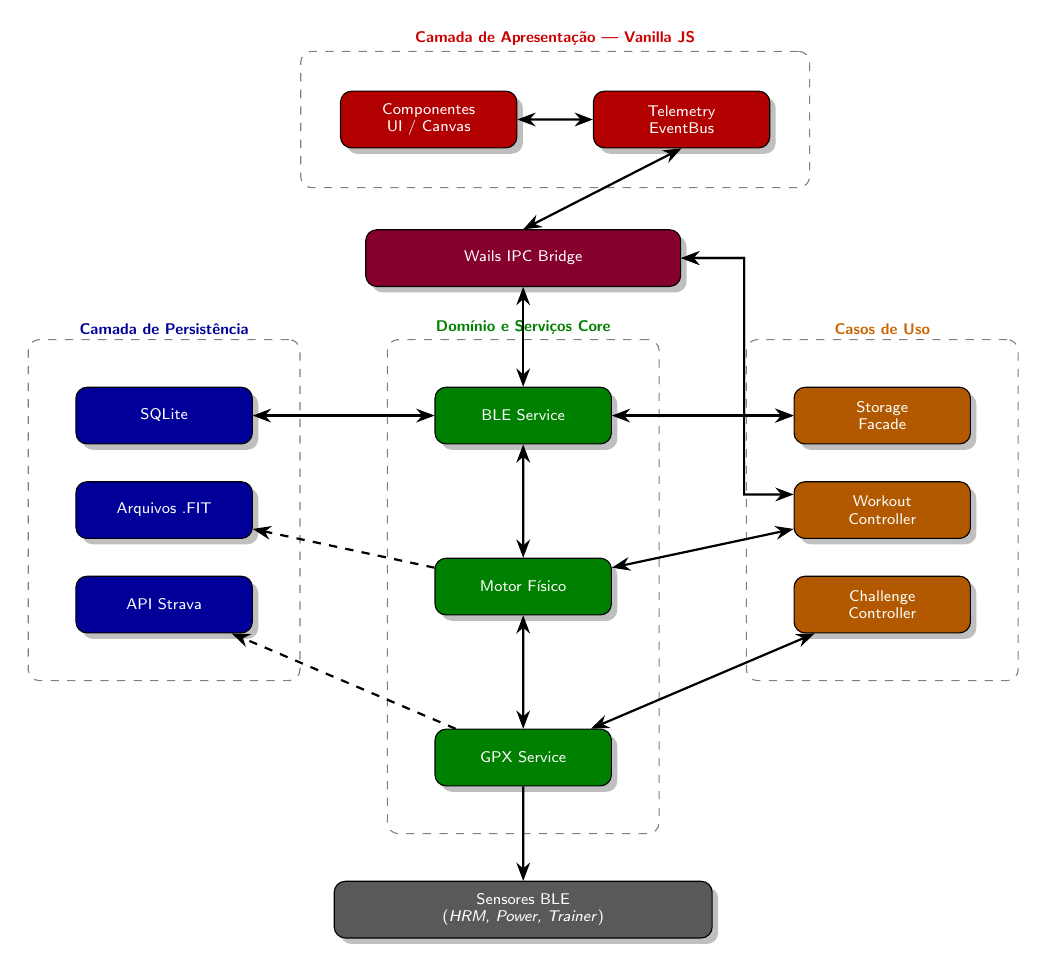
\begin{tikzpicture}[
      scale=0.8, % Escala levemente reduzida para dar mais fôlego
      every node/.style={transform shape},
      node distance=1.8cm and 1.5cm, % Distâncias aumentadas
      box/.style={rectangle, draw, rounded corners, minimum width=2.8cm, % Largura um pouco maior
        minimum height=0.9cm, align=center, font=\scriptsize\sffamily,
        text=white, drop shadow},
      layerbox/.style={rectangle, draw, dashed, black!50, rounded corners, thin},
      layerlabel/.style={font=\scriptsize\bfseries\sffamily, fill=white, inner sep=2pt},
      >=Stealth,
  ]

      % --- CAMADA DE APRESENTAÇÃO ---
      \node[box, fill=red!70!black] (ui) at (0, 4.2) {Componentes\\UI / Canvas};
      \node[box, fill=red!70!black] (teb) [right=1.2cm of ui] {Telemetry\\EventBus};
      
      \node[layerbox, inner sep=0.5cm, fit=(ui) (teb)] (frontlayer) {};
      \node[layerlabel, anchor=south, text=red!80!black] at (frontlayer.north) {Camada de Apresentação --- Vanilla JS};

      % --- WAILS IPC BRIDGE ---
      \node[box, fill=purple!70!black, minimum width=5.0cm, minimum height=0.9cm] (wails) at (1.5, 2.0) {Wails IPC Bridge};

      % --- DOMÍNIO E SERVIÇOS CORE ---
      \node[box, fill=green!50!black] (blesvc) at (1.5, -0.5) {BLE Service};
      \node[box, fill=green!50!black] (sim) [below=of blesvc] {Motor Físico};
      \node[box, fill=green!50!black] (gpx) [below=of sim] {GPX Service};
      
      \node[layerbox, inner sep=0.6cm, fit=(blesvc) (gpx)] (corelayer) {};
      \node[layerlabel, anchor=south, text=green!50!black] at (corelayer.north) {Domínio e Serviços Core};

      % --- CAMADA DE PERSISTÊNCIA ---
      \node[box, fill=blue!60!black] (sqlite) at (-4.2, -0.5) {SQLite};
      \node[box, fill=blue!60!black] (fit) at (-4.2, -2.0) {Arquivos .FIT};
      \node[box, fill=blue!60!black] (stravaapi) at (-4.2, -3.5) {API Strava};
      
      \node[layerbox, inner sep=0.6cm, fit=(sqlite) (stravaapi)] (persistlayer) {};
      \node[layerlabel, anchor=south, text=blue!60!black] at (persistlayer.north) {Camada de Persistência};

      % --- CASOS DE USO ---
      \node[box, fill=orange!70!black] (sf) at (7.2, -0.5) {Storage\\Facade};
      \node[box, fill=orange!70!black] (wc) at (7.2, -2.0) {Workout\\Controller};
      \node[box, fill=orange!70!black] (cc) at (7.2, -3.5) {Challenge\\Controller};
      
      \node[layerbox, inner sep=0.6cm, fit=(sf) (cc)] (uselayer) {};
      \node[layerlabel, anchor=south, text=orange!80!black] at (uselayer.north) {Casos de Uso};

      % --- HARDWARE ---
      \node[box, fill=gray!70!black, minimum width=6.0cm, minimum height=0.9cm] (sensors) [below=1.5cm of gpx] {Sensores BLE\\(\textit{HRM, Power, Trainer})};

      % --- CONEXÕES VERTICAIS E HORIZONTAIS ---
      \draw[<->, thick] (blesvc) -- (sim);
      \draw[<->, thick] (sim) -- (gpx);
      \draw[->, thick] (gpx) -- (sensors);
      
      % Conexões da Esquerda (Persistência)
      \draw[<->, thick] (blesvc) -- (sqlite);
      \draw[->, thick, dashed] (sim) -- (fit);
      \draw[->, thick, dashed] (gpx) -- (stravaapi);
      
      % Conexões da Direita (Casos de Uso)
      \draw[<->, thick] (sf) -- (blesvc);
      \draw[<->, thick] (wc) -- (sim);
      \draw[<->, thick] (cc) -- (gpx);
      
      % Conexões da Apresentação para a Bridge
      \draw[<->, thick] (teb) -- (ui);
      \draw[<->, thick] (teb.south) -- (wails.north);
      \draw[<->, thick] (wails.south) -- (blesvc.north);
      
      % Ponto de controle para as linhas
      \coordinate (p1) at ($(wails.east) + (1.0, 0)$);
      
      % Rota para StorageFacade: vai para a direita, desce contornando, e entra pelo lado OESTE
      \draw[<->, thick] (wails.east) -- (p1) |- (sf.west);
      
      % Rota para WorkoutController: entra pelo lado oeste, mas em um ponto mais baixo (170 graus)
      \draw[<->, thick] (wails.east) -- (p1) |- (wc.170);

  \end{tikzpicture}
\end{figure}

\section{Diagrama 2: Fluxo Sequencial de Telemetria de Baixa Latência}
\label{sec:diagrama-telemetria}

A simulação de ciclismo virtual exige uma comunicação de baixíssima latência. O diagrama de sequência da Figura~\ref{fig:telemetria} demonstra como os dados trafegam do sensor até a renderização gráfica no momento do pedal.

\begin{figure}[htbp]
  \centering
  \caption{Fluxo sequencial de telemetria em tempo real}
  \label{fig:telemetria}
  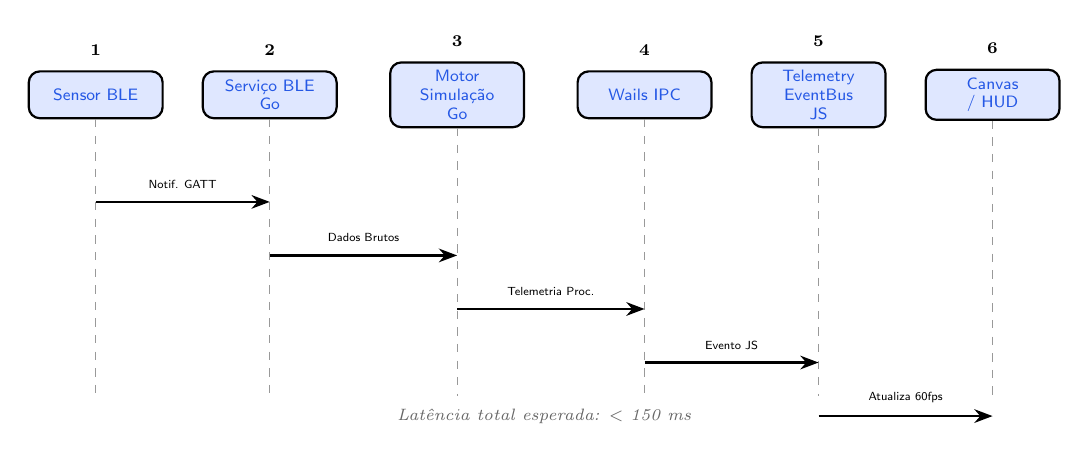
\begin{tikzpicture}[
      scale=0.85, every node/.style={transform shape},
      >=Stealth,
      actor/.style={rectangle, draw, rounded corners, minimum width=2.0cm,
        minimum height=0.7cm, align=center, font=\scriptsize\sffamily,
        fill=blueargus!15, text=blueargus!90!black, thick},
      edge node/.style={above, yshift=2pt, align=center, font=\tiny\sffamily},
      note/.style={font=\scriptsize\sffamily, align=center},
  ]

      % Lifelines
      \node[actor] (sensor) at (0,0) {Sensor BLE};
      \node[actor] (ble) at (2.6,0) {Serviço BLE\\Go};
      \node[actor] (sim) at (5.4,0) {Motor\\Simulação\\Go};
      \node[actor] (wails) at (8.2,0) {Wails IPC};
      \node[actor] (teb) at (10.8,0) {Telemetry\\EventBus\\JS};
      \node[actor] (canvas) at (13.4,0) {Canvas\\/ HUD};

      % Linhas tracejadas verticais
      \foreach \p in {sensor,ble,sim,wails,teb,canvas}
          \draw[dashed, black!40] (\p.south) -- (\p.south |- 0,-4.5);

      % Setas horizontais
      \draw[->, thick] (0,-1.6) -- node[edge node] {Notif. GATT} (2.6,-1.6);
      \draw[->, thick] (2.6,-2.4) -- node[edge node] {Dados Brutos} (5.4,-2.4);
      \draw[->, thick] (5.4,-3.2) -- node[edge node] {Telemetria Proc.} (8.2,-3.2);
      \draw[->, thick] (8.2,-4.0) -- node[edge node] {Evento JS} (10.8,-4.0);
      \draw[->, thick] (10.8,-4.8) -- node[edge node] {Atualiza 60fps} (13.4,-4.8);

      % Números sequenciais
      \node[note, font=\scriptsize\bfseries, above=3pt] at (sensor.north) {1};
      \node[note, font=\scriptsize\bfseries, above=3pt] at (ble.north) {2};
      \node[note, font=\scriptsize\bfseries, above=3pt] at (sim.north) {3};
      \node[note, font=\scriptsize\bfseries, above=3pt] at (wails.north) {4};
      \node[note, font=\scriptsize\bfseries, above=3pt] at (teb.north) {5};
      \node[note, font=\scriptsize\bfseries, above=3pt] at (canvas.north) {6};

      % Texto de latência
      \node[note, font=\scriptsize\itshape, text=black!60] at (6.7,-4.8) {Latência total esperada: \textless{} 150 ms};

  \end{tikzpicture}
\end{figure}

\section{Diagrama 3: Mapa Mental do Ecossistema e Funcionalidades}
\label{sec:diagrama-mapa-mental}

A Figura~\ref{fig:mapamental} apresenta o mapa mental do ecossistema Argus Cyclist, organizando as principais funcionalidades e suas inter-relações de forma totalmente legível.

\begin{figure}[htbp]
  \centering
  \caption{Mapa mental do ecossistema Argus Cyclist}
  \label{fig:mapamental}
  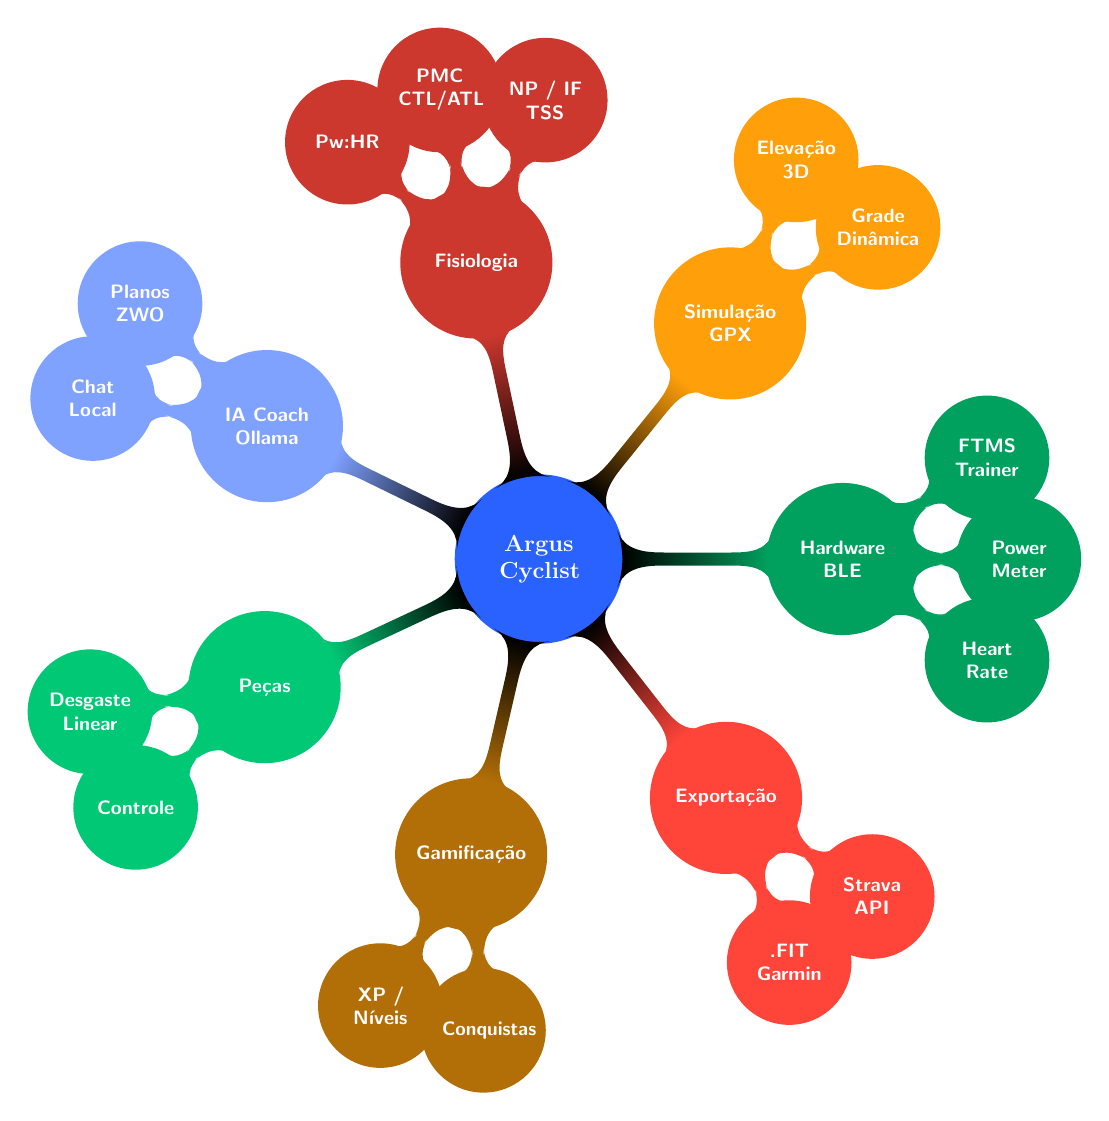
\begin{tikzpicture}[
      scale=0.7,
      transform shape,
      mindmap,
      every node/.style={concept, text=white, font=\sffamily\bfseries},
      root concept/.style={
        concept color=blueargus, 
        minimum size=3.0cm, 
        font=\large\bfseries,
        text width=2.8cm,
        align=center
      },
      level 1 concept/.append style={
        level distance=5.5cm, 
        minimum size=2.7cm, 
        font=\normalsize\bfseries,
        text width=2.0cm,
        align=center
      },
      level 2 concept/.append style={
        level distance=3.2cm, 
        minimum size=2.2cm, 
        font=\footnotesize\bfseries,
        text width=1.5cm,
        align=center
      },
  ]

        \node[root concept] {Argus\\Cyclist}
            % 1. Hardware BLE
            child[grow=0, concept color=greenargus!80!black] { node {Hardware\\BLE}
                child[grow=-35] { node {Heart\\Rate}}
                child[grow=0]   { node {Power\\Meter}}
                child[grow=35]  { node {FTMS\\Trainer}}
            }
            % 2. Simulação GPX
            child[grow=51.4, concept color=orangeargus] { node {Simulação\\GPX}
                child[grow=33.9] { node {Grade\\Dinâmica}}
                child[grow=68.9] { node {Elevação\\3D}}
            }
            % 3. Fisiologia
            child[grow=102.8, concept color=redargus!80!black] { node {Fisiologia}
                child[grow=67.8]  { node {NP / IF\\TSS}}
                child[grow=102.8] { node {PMC\\CTL/ATL}}
                child[grow=137.8] { node {Pw:HR}}
            }
            % 4. IA Coach Ollama
            child[grow=154.2, concept color=blueargus!60!white] { node {IA Coach\\Ollama}
                child[grow=136.7] { node {Planos\\ZWO}}
                child[grow=171.7] { node {Chat\\Local}}
            }
            % 5. Peças
            child[grow=205.7, concept color=greenargus] { node {Peças}
                child[grow=188.2] { node {Desgaste\\Linear}}
                child[grow=223.2] { node {Controle}}
            }
            % 6. Gamificação
            child[grow=257.1, concept color=orangeargus!70!black] { node {Gamificação}
                child[grow=239.6] { node {XP / Níveis}}
                child[grow=274.6] { node {Conquistas}}
            }
            % 7. Exportação
            child[grow=308.5, concept color=redargus] { node {Exportação}
                child[grow=291] { node {.FIT\\Garmin}}
                child[grow=326] { node {Strava\\API}}
            };
  \end{tikzpicture}
\end{figure}

% ====================================================================
%  SEÇÃO 7 — CONCLUSÃO
% ====================================================================
\chapter{CONCLUSÃO}
\label{sec:conclusao}

O desenvolvimento do Argus Cyclist demonstra a viabilidade técnica de uma plataforma de ciclismo virtual de código aberto, multiplataforma e orientada ao processamento local. O projeto diferencia-se por combinar simulação física em tempo real, análise fisiológica avançada, integração com dispositivos BLE e recursos de inteligência artificial executados localmente, preservando a privacidade dos usuários e reduzindo dependências de infraestrutura em nuvem. Adicionalmente, o sistema de rastreamento de desgaste de componentes oferece uma ferramenta prática de manutenção preventiva, preenchendo uma lacuna não endereçada pelas plataformas comerciais existentes.

Além da contribuição tecnológica, a proposta possui relevância social significativa ao democratizar o acesso ao treinamento esportivo científico, especialmente para atletas amadores e usuários com limitações financeiras ou computacionais. Dessa forma, o Argus Cyclist consolida-se como uma alternativa inovadora às soluções proprietárias do mercado, unindo acessibilidade, desempenho e liberdade tecnológica.

\postextual

% ====================================================================
%  REFERÊNCIAS BIBLIOGRÁFICAS
% ====================================================================
\begin{thebibliography}{9}
    \bibitem{bluetooth2017}
    BLUETOOTH SIG.
    \textbf{Fitness Machine Service (FTMS) Specification v1.0}.
    Bluetooth Special Interest Group, 2017.
    Disponível em: \url{https://www.bluetooth.com/specifications/specs/}.

    \bibitem{garmin2024}
    GARMIN.
    \textbf{FIT SDK (Flexible and Interoperable Data Transfer)}.
    ANT+ Alliance, Garmin Canada, 2024.
    Disponível em: \url{https://developer.garmin.com/fit/overview/}.

    \bibitem{martin1998}
    MARTIN, J. C. \textit{et al.}
    Validation of a Mathematical Model for Road Cycling Power.
    \textbf{Journal of Applied Biomechanics}, Human Kinetics, v.~14, n.~3,
    p.~276--291, 1998.

    \bibitem{coggan2010}
    COGGAN, A.
    \textbf{Training and Racing with a Power Meter}.
    2.~ed. Boulder, CO: VeloPress, 2010.

    \bibitem{echarts2024}
    ECHARTS.
    \textbf{Apache ECharts Documentation v5}.
    Apache Software Foundation, 2024.
    Disponível em: \url{https://echarts.apache.org/}.

    \bibitem{gpx2004}
    TOPOGRAFIX.
    \textbf{GPX: GPS Exchange Format v1.1}.
    2004.
    Disponível em: \url{https://www.topografix.com/gpx.asp}.

    \bibitem{maplibre2024}
    MAPLIBRE.
    \textbf{MapLibre GL JS Documentation v4}.
    MapLibre Community, 2024.
    Disponível em: \url{https://maplibre.org/}.

    \bibitem{ollama2024}
    OLLAMA.
    \textbf{Ollama: Local LLM Inference Platform}.
    2024.
    Disponível em: \url{https://ollama.ai/}.

    \bibitem{sqlite2024}
    SQLITE CONSORTIUM.
    \textbf{SQLite Documentation v3}.
    2024.
    Disponível em: \url{https://sqlite.org/}.

    \bibitem{strava2025}
    STRAVA API.
    \textbf{Strava Developers API Reference v3}.
    Strava Inc., 2025.
    Disponível em: \url{https://developers.strava.com/}.

    \bibitem{tinygo2024}
    TINYGO.
    \textbf{TinyGo Bluetooth: BLE Library for Go}.
    2024.
    Disponível em: \url{https://tinygo.org/x/bluetooth/}.

    \bibitem{wails2024}
    WAILS.
    \textbf{Wails: Create Beautiful Desktop Applications using Go and HTML/CSS/JS v2}.
    Wails Project, 2024.
    Disponível em: \url{https://wails.io/}.

    \bibitem{capacitor2024}
    CAPACITOR.
    \textbf{Capacitor: Cross-platform Native Runtime for Web Apps v5}.
    Ionic Project, 2024.
    Disponível em: \url{https://capacitorjs.com/}.
\end{thebibliography}

\end{document}